\documentclass[tikz]{standalone}

%: === FONT === (((
\usepackage{fontspec}
\setmainfont[
  BoldFont       = bodonibi,
	ItalicFont     = Century modern italic2.ttf,
	BoldItalicFont = bodonibi,
	SmallCapsFont  = lmromancaps10-regular.otf
]{Century_modern.ttf}
\DeclareSymbolFont{italics}{\encodingdefault}{\rmdefault}{m}{it}
\DeclareSymbolFontAlphabet{\mathit}{italics}
\ExplSyntaxOn
\int_step_inline:nnnn { `A } { 1 } { `Z }
 {  \exp_args:Nf \DeclareMathSymbol{\char_generate:nn{#1}{11}}{\mathalpha}{italics}{#1} }
\int_step_inline:nnnn { `a } { 1 } { `z } {  \exp_args:Nf \DeclareMathSymbol{\char_generate:nn{#1}{11}}{\mathalpha}{italics}{#1}}
\ExplSyntaxOff
% )))

\begin{document}

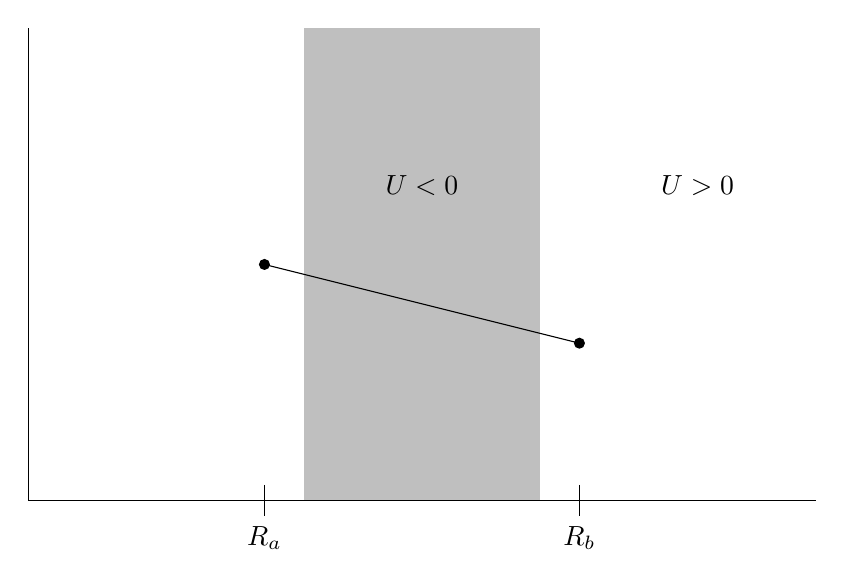
\begin{tikzpicture}[>=latex]

	\fill [gray!50] (3.5,0) rectangle (6.5,6);
	\draw (0,0) -- (10,0);
	\draw (0,0) -- (0,6);
	\draw (3,0.2) -- (3,-0.2) node [below] {\(R_a\)};
	\draw (7,0.2) -- (7,-0.2) node [below] {\(R_b\)};
	\node at (8.5,4) {\(U >0\) };
	\node at (5,4) {\(U < 0\)};
	\fill (3,3) circle (2pt);
	\fill (7,2) circle (2pt);
	\draw (3,3) -- (7,2);

\end{tikzpicture}

\end{document}
